% Separate evidence revision; the original LDraw-2 manuscript is immutable.
\documentclass[10pt,twocolumn,letterpaper]{article}
\usepackage[review]{cvpr}
\usepackage{times,graphicx,amsmath,amssymb,booktabs,tabularx}
\usepackage[T1]{fontenc}
\usepackage{microtype}
\definecolor{cvprblue}{rgb}{0.15,0.43,0.64}
\usepackage[pagebackref,breaklinks,colorlinks,allcolors=cvprblue]{hyperref}
\def\paperID{Draft}
\def\confName{CVPR}
\def\confYear{2026}
\newcommand{\EvSources}{24}
\newcommand{\EvParts}{15,334}
\newcommand{\EvTasks}{617}
\newcommand{\EvVisual}{140}
\newcommand{\EvStructural}{146}
\newcommand{\EvControls}{290}
\newcommand{\EvConstant}{41}
\newcommand{\EvNodeHits}{63}
\newcommand{\EvGraphN}{73}
\newcommand{\EvNodeMicro}{86.30}
\newcommand{\EvNodeMacro}{83.75}
\newcommand{\EvNodeLo}{72.92}
\newcommand{\EvNodeHi}{93.12}
\newcommand{\EvPositiveDeficit}{10}
\newcommand{\EvPositiveSources}{9}
\newcommand{\EvChallengeObs}{219}
\newcommand{\EvChallengePairs}{146}
\newcommand{\EvChallengeUp}{37}
\newcommand{\EvChallengeDown}{36}
\newcommand{\EvChallengeSame}{73}
\newcommand{\EvDegreeMatched}{12}
\newcommand{\EvDegreeGaps}{61}
\newcommand{\EvFixedMacro}{61.11}
\newcommand{\EvFixedLo}{46.32}
\newcommand{\EvFixedHi}{75.07}
\newcommand{\EvFrozenFiles}{2,616}
\newcommand{\EvPlannedRuns}{84}
\newcommand{\EvPhysicalPending}{573}
\newcommand{\EvOtherPending}{111}
\newcommand{\EvColorN}{73}
\newcommand{\EvTypeN}{67}
\newcommand{\EvStepN}{17}
\newcommand{\EvLimitN}{24}
\newcommand{\EvRestoreN}{58}

\title{Following Evidence About the Same Part:\\
An Instance-Aligned Benchmark on LDraw Assemblies}
\author{Anonymous submission}
\begin{document}
\maketitle

\begin{abstract}
A correct answer about a part does not establish that a vision-language
model followed the evidence identifying that part. The answer may follow
a prior, persist after relevant evidence changes, or change under an
irrelevant display perturbation. We introduce BrickAtlas, an
instance-aligned measurement protocol on \EvSources{} human-authored
LDraw assemblies with \EvParts{} placed parts. Its main question is whether
answers about the same target correctly follow changed visual evidence
and remain correct under specified semantic invariances. The
\EvTasks{}-item resource separates \EvVisual{} visual questions,
\EvStructural{} graph questions and two classes of controls. Paired
observations bind canonical identities, exact inputs, condition-specific
gold answers and answerability decisions. New-evidence accuracy and
paired both-correct distinguish adaptation from disruption.
An audit of the unchanged graph questions illustrates the need:
counting nodes alone attains \EvNodeMicro\% accuracy, but zero
both-correct on answer-changing graph pairs, while a graph algorithm
solves both sides. A separate matched-graph extension controls additional
surface statistics. We report verified corpus and algorithmic evidence;
visual model comparisons and human answerability review remain unrun.
The contribution is a reproducible resource and falsifiable protocol,
not a completed model ranking.
\end{abstract}

\section{Introduction}
In a dense assembly, two pieces can share geometry while differing in
color, position or identity. A question about one piece therefore asks
more than whether a familiar shape is present: an answer must remain
bound to the designated instance. If the visible assignment of labels
to pieces changes, a model should follow the new evidence. If only the
names used to identify pieces change consistently, the semantic answer
should remain correct. Ordinary accuracy observes neither distinction.

This motivates our primary research question: \emph{for the same
identified part in an original assembly, do answers correctly follow
task-relevant visual changes and remain correct under specified
answer-preserving changes?} We study Color and Part-type separately.
Two supporting questions concern the total effect of hiding
non-operands at a fixed camera and whether graph answers follow
relations beyond elementary input statistics.

Human-authored LDraw models~\cite{ldraw} provide useful test conditions:
repeated instances, densely nested assemblies, author step records and
geometry at preserved source poses. Instance identity links these
assets without requiring them all in one question.
Figure~\ref{fig:identity} illustrates the distinction. A visual question
uses a numbered image; a separate graph question uses an explicit edge
list; a visibility edit uses declared actions. Shared identity permits
controlled inspection, but does not imply a within-item multimodal
reasoning chain.

\begin{figure*}[t]
\centering
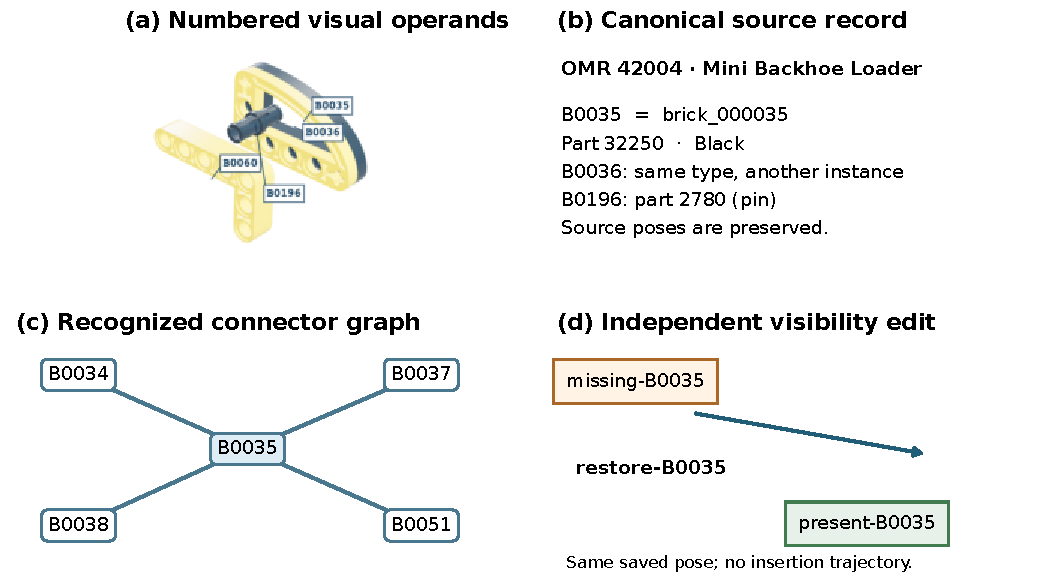
\includegraphics[width=\textwidth]{figures/instance-alignment.pdf}
\caption{One source instance, separately scored contracts. In OMR 42004,
B0035 is a black part 32250 and B0036 is another instance of the same
type. (a) Detail from the numbered operand image; other source parts
are hidden, with remaining poses unchanged. (b) Canonical source
records disambiguate repeated types. (c) Recognized axle edges link
B0035 to four other instances; this schematic does not depict spatial
placement. (d) An independent action restores visibility at the saved
pose. Records and graph facts are not supplied to the visual question.
The links support inspection across tasks, not a single cross-module
inference chain.}
\label{fig:identity}
\end{figure*}

Related resources already supply important ingredients.
BrickNet~\cite{kulits2026bricknet} has instance and connector graphs;
LEGO-Puzzles~\cite{tang2025legopuzzles} uses editable scenes and
step-consistent renders; PhyBlock~\cite{ma2025phyblock} combines
scene identity, dependencies and simulated assembly. Our distinction
is the explicitly paired measurement: an identified target, exact
observations, two semantic golds, and a decision on whether each
observation makes the question answerable. A change in old-gold
accuracy alone cannot establish that an answer followed new evidence.

The present empirical evidence is algorithmic. On all \EvGraphN{}
natural deletion questions, a predictor that ignores edges and returns
the node count minus one answers \EvNodeHits{} correctly. On the
corresponding fixed-node, answer-changing pairs it answers neither
pair jointly correctly; connected-component algorithms solve both.
This post-hoc replication exposes a concrete interpretive gap between
high accuracy and evidence following. It is not a result about a
learned model.

Our contributions are threefold. First, we make same-instance visual
evidence following measurable on unchanged source assemblies, with
modular structural and execution controls. Second, we define paired
semantic measures and source-balanced estimates that separate
correct adaptation, stable error and information withdrawal.
Third, we supply an audited natural distribution and an independently
verified hypothetical graph challenge. The full question index,
input provenance, baselines and executable analysis accompany the
resource. The visual research question remains open until exact-input
human review and genuine model responses are available.

\section{Related Protocols}
\begin{table*}[t]
\centering\small
\caption{Related protocols and the evidence they measure. Comparisons use
BrickNet's CVPR 2026 paper, LEGO-Puzzles arXiv v3 and PhyBlock arXiv v2.
``Not reported'' refers to the specific paired VQA estimand, not an inability
to implement it. Full page- and code-level evidence is in the supplement.}
\label{tab:related}
\begin{tabularx}{\textwidth}{@{}p{1.75cm}XXX@{}}
\toprule
Protocol & Instance alignment and observations & Controlled comparison &
Measured outcome\\
\midrule
BrickNet~\cite{kulits2026bricknet} &
Graph-local part and connector IDs; generates programs from a start token
or caption. &
Graph/pose representations, sampling and training ablations. &
Parse/connectivity and collision validity; render--text agreement.
Our paired VQA estimand is not reported.\\
LEGO-Puzzles~\cite{tang2025legopuzzles} &
Image tokens, option labels and arrows; multiple current/target/part images
support spatial and sequential questions. &
Fixed camera across steps; editable scene attributes; step length and
prompt comparisons. &
VQA/ordering accuracy and human-rated image generation.
Our paired VQA estimand is not reported.\\
PhyBlock~\cite{ma2025phyblock} &
Scene-instance IDs and dependencies; reusable candidate IDs in planning;
target/candidate images and optional feedback. &
Pose-constrained/topology-oriented scoring, stepwise feedback and
simulated perturbations. &
AOV step precision/recall and physical VQA accuracy.
Our paired VQA estimand is not reported.\\
BrickAtlas &
Canonical instance linked to images, records, graphs and display edits;
each item has one declared contract. &
Same-target fact change, semantic invariance and evidence withdrawal,
with separately bound golds. &
New-evidence accuracy and paired both-correct; source-cluster contrasts.
Learned-model results remain unrun.\\
\bottomrule
\end{tabularx}
\end{table*}

Compositional VQA resources such as CLEVR~\cite{johnson2017clevr} and
GQA~\cite{hudson2019gqa} motivate specifying what operations and evidence
a question requires. Our focus is narrower: following evidence about
an identified part under paired observations, with separate controls
for source lookups, graph operations and display actions.
Table~\ref{tab:related} compares the three closest assembly protocols.
The supplement records paper pages, exact versions and inspected
official code symbols.

BrickNet generates graph-backed programs and measures parse,
connectivity, collision and perceptual properties. Distinct placed
instances and connectors are already explicit in its representation.
LEGO-Puzzles evaluates spatial and sequential VQA, sometimes jointly
using current, target and part images. Its v3 protocol includes
three-annotator verification and editable rendered scenes.
PhyBlock evaluates planning against legal dependency orders and
physical understanding through static and dynamic questions. Its scene
records identify target instances, while candidate IDs in planning
can denote reusable block variants. These are substantial capabilities,
not absences that our use of IDs resolves.

The same-target, new-gold and both-correct VQA estimands used here are
not reported in these pinned versions. Their assets could support
extensions with this protocol. Adding IDs and templates can establish
which source entity a question concerns; it does not by itself specify
how the answer should change for a second rendered observation,
whether that observation is decidable, or which semantic transition a
raw response exhibits. Those additional records define the object of
measurement in BrickAtlas.

\section{Benchmark and Observation Contracts}
\subsection{Source assemblies and identity}
The resource contains \EvSources{} original assemblies,
\EvParts{} placed instances and \EvTasks{} questions. Source files,
part transforms and original gold answers are preserved. Each canonical
identity combines a source hash with an instance ID. A display label
such as B0035 is unique within its source, not across the corpus.
Repeated part numbers remain different instances. Source-size bands
D1--D4 describe corpus scale; they are not validated cognitive
difficulty levels.

The images use actual LDraw geometry. Hiding non-operands and replaying
visibility changes do not relocate any part. Such partial observations
can omit supporting pieces; they represent access to an unchanged
assembly, not a proposed physical arrangement. Recognized connector
relations establish a limited graph, not exhaustive contact, gravity
stability or mechanical feasibility. Unresolved physical candidates
are retained for review.

\subsection{Task roles and scope}
Every item has one declared model-visible contract: a numbered image
(V), selected source records (S), explicit graph evidence (G), or
facts and discrete display actions (E). The scorer's source records,
references and alternate gold are separate from the request.
No family is presented as a full perception-to-assembly pipeline.

The four reporting roles are disjoint. Core visual questions comprise
\EvColorN{} Color and \EvTypeN{} Part-type items. Structural evidence
comprises Neighbors and Graph deletion, \EvGraphN{} each. The
\EvControls{} nonconstant controls test coordinate distance, interface
records, coverage flags, author-step lookup and visibility restoration.
The \EvConstant{} constant controls contain \EvLimitN{} evidence-limit
responses and \EvStepN{} fixed step programs. All items remain in the
complete report; no composite capability ranking mixes these roles.

Color selects the rendered target's color category. Part-type asks
which numbered candidate shares its source type while ignoring color
and pose. Near-identical geometry can make a source-derived type answer
visually undecidable; exact-input QA must resolve that boundary.
Neighbors returns an exact set from the supplied local graph.
Graph deletion returns the number of connected components after
removing the target, counting isolated survivors and deduplicating
undirected edges.

\begin{figure*}[t]
\centering
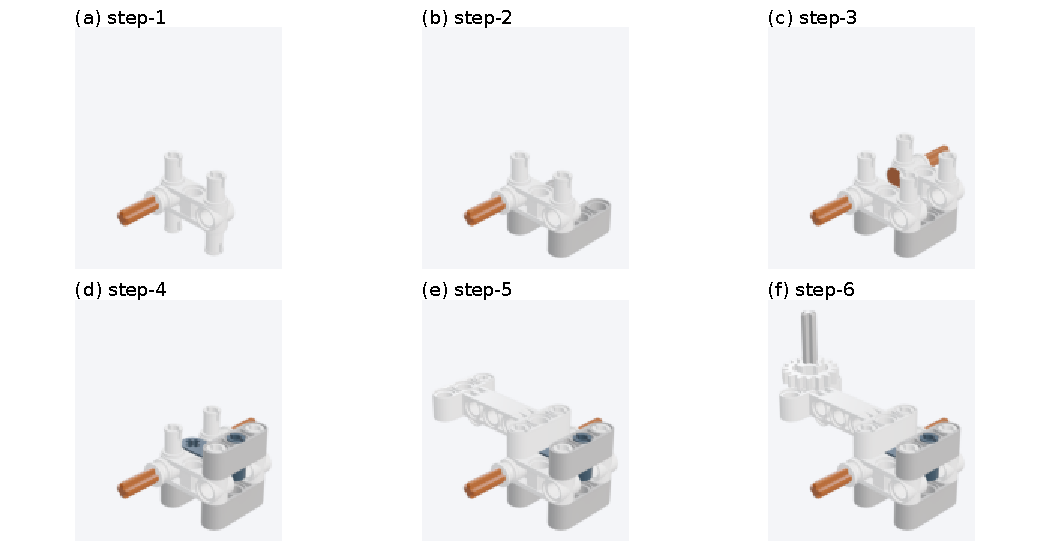
\includegraphics[width=\textwidth]{figures/given-order-replay.pdf}
\caption{Given-order visibility replay for the supplied author window
of set 42102. Panels (a)--(f) show the accepted actions step-1 through
step-6, with a common paper crop and original source transforms.
The program is supplied by the contract and is constant across this
control family. The frames demonstrate action-to-display correspondence;
they do not establish discovery of an assembly order, an insertion
trajectory or stability.}
\label{fig:replay}
\end{figure*}

Execution controls expose preconditions, forbidden facts, effects,
budget and goals. A legal restoration makes one hidden instance visible
at its saved pose. The given-order replay in Figure~\ref{fig:replay}
follows six declared actions. Invalid actions do not change the state.
These controls measure contract execution and output compliance,
not mechanical planning.

\subsection{Paired observations}
Let a pair be $(i,s,o_A,o_B,y_A,y_B,\tau)$, where $i$ is the parent
question, $s$ the source, $o$ the exact observation, $y$ its semantic
gold and $\tau$ its truth policy. We distinguish three policies.
\emph{Fact change} assigns two distinct observation-conditioned
answers. \emph{Semantic invariance} retains the canonical answer after
mapping display labels back to identities. \emph{Information withdrawal}
retains the original gold for a dependency comparison while removing
evidence needed to infer it.

The primary fact-change comparison pairs operand-only with wrong-image.
For Part-type, a displayed candidate-label swap changes which option
identifies the matching geometry. For Color, a donor image provides
different visual content; shape can change too, so this is not a
color-only causal intervention. Original source-gold scores remain
available as auxiliary dependency statistics. The new analysis adds
the image-conditioned gold without overwriting those scores.

Invariance comparisons cover consistent ID renaming, camera changes
and type-preserving color appearance changes. The existing ID
permutation uses longer labels and can move text boxes, so it measures
stability under naming and display changes rather than a pure
identity-only effect. Semantic invariance is necessary but insufficient
for visual answerability: a changed view can hide a distinguishing
feature.

\section{Measurement Validity}
\subsection{Priors and retained denominators}
\begin{figure*}[t]
\centering

\includegraphics[width=\textwidth]{figures/answer-priors.pdf}
\caption{Two different corpus diagnostics. (a) The frequency of the
most common global semantic answer exposes category and fixed-output
priors. (b) Exact source-scoped answers include the source and instance
identity; low repetition is partly a consequence of that key space.
The panels use separate scales and are not comparable measures of
difficulty. In particular, the global constant-answer prior for graph
deletion is weaker than the input-conditioned node-count baseline in
Table~\ref{tab:algorithms}. These are corpus counts, not model scores.}
\label{fig:priors}
\end{figure*}

Answer concentration has different meanings across families
(Figure~\ref{fig:priors}). A frequent color category supports a global
constant predictor. An answer keyed by a source-specific instance rarely
repeats even if the operation is trivial. A small exact-key repetition
rate therefore does not certify reasoning difficulty.

Graph deletion illustrates a stronger input-conditioned prior. For
target $t$, let $n'$ be the number of surviving nodes and $c'$ their
component count. Define the analysis-only deficit
\begin{equation}
d=n'-c'.
\end{equation}
If $d=0$, returning $|V|-1$ is correct without reading any edge.
We retain all questions and report both $d=0$ and $d>0$ strata.
These strata describe the corpus and never enter model prompts.
Removing the easy stratum would change the target distribution.

\subsection{Independent gold and input checks}
Node-only prediction accepts only a public node list. A later scoring
phase joins those saved predictions with references and graph
statistics. Breadth-first search (BFS) and an independently implemented
union-find procedure agree on every original and intervened deletion
gold. They explicitly handle duplicate edges, isolated nodes and
target deletion. Graph oracles validate supplied evidence; they do
not certify that all physical connections were recognized.

Each paired record binds source and dataset hashes, exact model
revision, adapter, prompt, both request bodies, normalized predictions,
gold provenance and truth policy. Validation reconstructs the wire
request and parses the saved raw response. It rejects mismatched
revisions and duplicate pairs. A missing B response remains a failed
observation in the declared denominator; it is not removed by taking
the intersection of successful requests.

\subsection{Answerability and quality decisions}
Visual accuracy is interpretable only for inputs that support the
question. Review binds the actual image bytes and dimensions sent in
the request, not a higher-resolution source render or an extra view.
A paired visual comparison requires independent answerability decisions
for both observations. Pending, failed and access-difference cases
remain explicitly enumerated alongside the full-denominator result.
No model-dependent filtering is permitted.

The current review inventory contains \EvVisual{} visual items,
\EvOtherPending{} other flagged items and \EvPhysicalPending{}
source-local intersection candidates. A candidate can reflect intended
mating, mesh approximation, a source defect or an unresolved case;
it is not automatically a collision error. Software validation and the
paper's enlargements do not count as human certification.

\section{Evidence-Following Evaluation}
\subsection{Measures and aggregation}
For $N$ fixed pairs with normalized predictions $p_A,p_B$, the primary
fact-change measures are
\begin{align}
\mathrm{NewAcc}&=\frac{1}{N}\sum_i [p_{Bi}=y_{Bi}],\\
\mathrm{Both}&=\frac{1}{N}\sum_i
 [p_{Ai}=y_{Ai}]\,[p_{Bi}=y_{Bi}].
\end{align}
The optional conditional adaptation rate divides the same both-correct
numerator by $\sum_i[p_{Ai}=y_{Ai}]$. A zero conditional denominator
returns undefined, not zero. We always retain the unconditional rates
and display the conditional denominator.

For wrong-image, B outcomes partition into the new answer, the old
answer, another legal answer, and invalid or missing output.
For invariance, we report both correct, A-only correct, B-only correct,
both wrong with the same semantic answer, and both wrong with different
answers. Invalid outputs carry a separate reason and do not become
evidence of semantic agreement. Set answers are order-independent,
but illegal duplicates are not silently repaired; action answers use
the executable contract.

These measures resolve two ambiguities. A model can be correct on
both graphs while its accuracy difference is zero. Conversely, an
answer can change without either answer being correct. A consistently
wrong answer is also distinct from correct retention. Output changes
and old-gold accuracy remain useful auxiliary statistics, not substitutes
for paired correctness.

For pair-level values $z_{spv}$, the source-balanced estimate is
\begin{equation}
\widehat{\mu}=\frac{1}{|S|}\sum_{s\in S}
 \frac{1}{|P_s|}\sum_{p\in P_s}
 \frac{1}{|V_{sp}|}\sum_{v\in V_{sp}}z_{spv}.
\end{equation}
Thus variants first average within a parent, parents within a source,
then sources equally. We also report micro rates, parent counts and
source counts. A family absent from a source contributes no zero.
Percentile 95\% intervals use 10,000 source-cluster bootstrap draws
with seed 20260919. Model--baseline differences are computed on the
same paired items before resampling. Repeated observations do not
increase the number of independent sources.

\subsection{Primary question: visual evidence following}
\begin{table}[t]
\centering\small
\caption{Core visual reporting, with fixed family denominators.
No validated learned-model results are available: ``--'' means not
run, never zero. Human answerability is pending. Family-specific
results replace an all-task capability ranking.}
\label{tab:visual}
\begin{tabular}{lrrr}
\toprule
Family / model & $N$ & Sources & Source macro (\%) \\
\midrule
Color & 73 & 24 & -- \\
Part-type & 67 & 24 & -- \\
\bottomrule
\end{tabular}

\end{table}

The visual experiment asks whether new-image accuracy and both-correct
remain high for a fact change, and whether correct retention survives
specified invariances. Color and Part-type remain separate
(Table~\ref{tab:visual}). Lower accuracy against the old gold is
insufficient: it can represent adaptation, confusion or invalid output.
The four B-outcome categories reveal which occurred.

A concrete source example makes the contrast testable. In OMR 42004,
B0035 and B0036 share part type 32250, while B0196 is a pin.
With fixed options A:B0196 and C:B0036, the operand image's gold is C.
Swapping the visible B0036/B0196 labels makes the image-conditioned
gold A. The source CAD remains unchanged. C$\rightarrow$A is the
desired paired response; C$\rightarrow$C retains the old answer;
C$\rightarrow$B is another legal error. These are scoring examples,
not observed model predictions. The supplement includes both actual
images and their provenance.

The result index currently contains only unrun learned-model records.
Exact requests and alternate gold mappings are validated, but no
claim about visual model sensitivity, adaptation or robustness follows
from that check. The protocol can falsify evidence following once
genuine responses and condition-specific QA exist.

\subsection{Supporting question: background and view access}
\begin{figure*}[t]
\centering
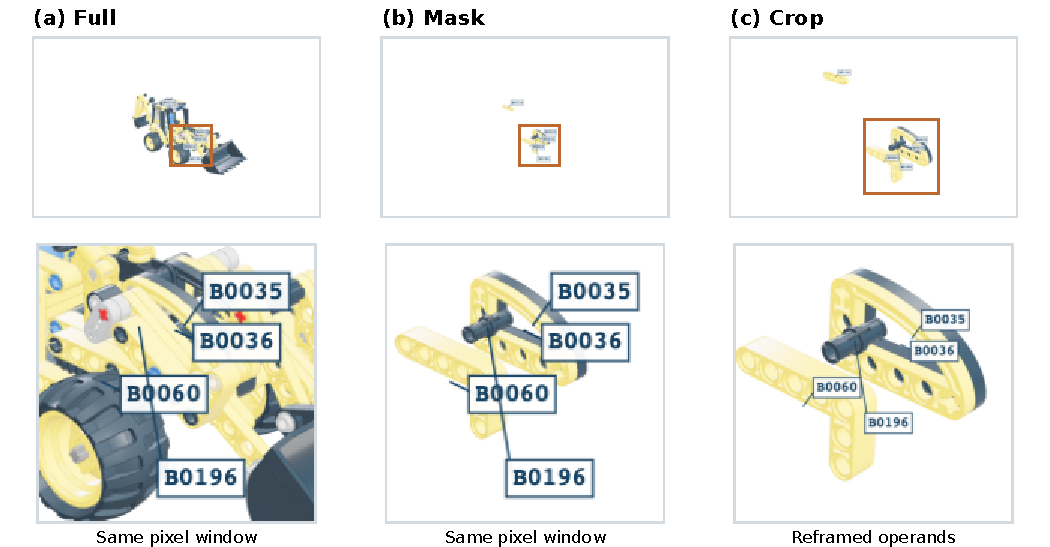
\includegraphics[width=\textwidth]{figures/full-mask-crop.pdf}
\caption{Full / Mask / Crop for the same Part-type item.
Top: each original frame with the paper's detail window.
Bottom: enlarged details; Full and Mask use exactly the same pixel
rectangle. Full/Mask fix camera, scale, lighting and label placement,
while hiding non-operands can reveal occluded surfaces. The comparison
measures the total effect of this access change, not pure attention.
Crop additionally reframes the operands. All enlargements and orange
boxes exist only in the paper and are not model inputs. Original poses
are preserved, and answerability remains subject to exact-input QA.}
\label{fig:access}
\end{figure*}

Full-scene versus background-mask holds camera, scale, lighting and
label placement fixed (Figure~\ref{fig:access}). Its primary contrast
is the paired source-macro accuracy difference. Hiding non-operands
both removes context and may expose surfaces; those effects are not
separately identified. Crop changes magnification and cannot isolate
background effects. Operand-only versus multi-view measures access
to two fixed views, not adaptive exploration.

For each visual comparison, the release preserves the planned set,
the jointly decidable set, and reasons for pending or excluded
interpretation. Differences are accompanied by source counts and
clustered intervals. An interval containing zero does not establish
equivalence. No unsegmented screenshot is used to invent an occlusion
percentage or projected target area. With no learned-model responses,
the direction and magnitude of these access effects remain unknown.

\subsection{Supporting question: graph evidence beyond priors}
\begin{table}[t]
\centering\small
\caption{Structural family reporting on the natural distribution.
``--'' means learned-model inference is unrun. Deletion requires the
algorithmic controls in Table~\ref{tab:algorithms} and paired success;
an ordinary family score alone is insufficient.}
\label{tab:structural}
\begin{tabular}{lrrr}
\toprule
Family / model & $N$ & Sources & Source macro (\%) \\
\midrule
Neighbors & 73 & 24 & -- \\
Graph deletion & 73 & 24 & -- \\
\bottomrule
\end{tabular}

\end{table}
\begin{table*}[t]
\centering\small
\caption{Measured algorithmic controls on the unchanged \EvGraphN{}
deletion questions and their original/intervened pairs
(\EvSources{} sources). Both is the source-macro rate of answering
each pair correctly. Natural source-macro intervals are 95\%
source-cluster intervals, reported in the text and supplement.
These are executable baselines, not learned-model results.}
\label{tab:algorithms}
\begin{tabular}{lrrr}
\toprule
Algorithmic baseline & Micro (\%) & Source macro (\%) & Both (\%) \\
\midrule
Node count only & 86.30 & 83.75 & 0.00 \\
Always four & 60.27 & 61.11 & 0.00 \\
BFS / union-find & 100.00 & 100.00 & 100.00 \\
\bottomrule
\end{tabular}

\end{table*}

The node-only baseline reaches \EvNodeHits/\EvGraphN{}
(\EvNodeMicro\% micro; \EvNodeMacro\% source macro,
95\% interval [\EvNodeLo, \EvNodeHi]).
The interval concerns sampling variation across these source clusters;
the exact corpus count itself has no sampling uncertainty.
Only \EvPositiveDeficit{} items from \EvPositiveSources{} sources
have positive deficit. This small stratum limits conclusions about
natural surviving-edge difficulty.

The existing intervention adds one edge between surviving components,
keeping the node set fixed and reducing the gold component count by
one. Table~\ref{tab:algorithms} shows zero both-correct for node-only
and always-four predictors, versus 100\% for BFS/union-find. The
contrast establishes that ordinary high accuracy on this distribution
can be obtained without consulting the defining relations.
It does not establish that any learned model uses this shortcut.
The node-prior concern was already known before this revision;
the replication and stratification are post-hoc audits.

To control additional surface statistics, a separate extension fixes
three observations per parent: a hypothetical anchor, an
answer-changing partner, and an isomorphic answer-preserving variant.
Its \EvChallengeObs{} observations form \EvChallengePairs{} pairs:
\EvChallengeUp{} increases, \EvChallengeDown{} decreases and
\EvChallengeSame{} unchanged answers. All pairs match node set,
unique edge count and target degree. \EvDegreeMatched{} answer-changing pairs
also match the surviving degree sequence; the other \EvDegreeGaps{} parents have
only four or five survivors, for which the declared templates do not
provide that match.

For six or more survivors, a six-cycle versus two triangles has
different component counts despite identical per-node degrees.
For four or five survivors, a path versus triangle-plus-isolates
matches counts but not degrees. Additional survivors are isolated.
These graphs deliberately change the evidence distribution and are
labeled hypothetical; they are not newly inferred source connections.
They add no source and never replace the natural questions.

All extension golds agree under independent graph algorithms.
Rules and shuffled opaque observation IDs were fixed before new
model responses. Each observation receives a fresh request without
the transformation or answer direction. The extension's algorithmic
verification is complete, while learned-model inference is unrun.
Natural, original-intervention and matched-challenge results must
remain separately reported.

\section{Discussion and Resource Use}
This resource isolates a modest but important requirement: answering
about an identified part should follow the evidence made available
for that question. Preserved source identity supports controlled
observations; condition-specific gold and raw semantic responses make
correct adaptation distinguishable from disturbance. The algorithmic
audit demonstrates the interpretive value of that distinction on the
present graph distribution.

Several limits determine the scope of future conclusions. The corpus
has only \EvSources{} human-authored sources, and shared parts or
authoring conventions can create dependence beyond a source cluster.
Visual answerability is unresolved. Connector coverage is incomplete,
display edits do not model forces, and the matched challenge is an
artificial graph distribution. Modular task scores cannot locate a
model's internal cognitive failure or demonstrate end-to-end assembly.

The supplement contains all \EvTasks{} questions and golds for audit,
full family/control tables, source coverage, protocol evidence and
failure cases. Reference-bearing materials are evaluator resources,
not inference inputs. Future training splits must keep every source
and all its views and variants together. Reusing public sources also
requires explicit contamination and source-rights review.

The analysis separates unavailable evidence from measured zero.
API errors, timeouts, refusals and invalid outputs remain in the
denominator with distinct reasons. A completed result enters the
paper only after its manifest, raw receipts, semantic scoring and
sample counts pass validation. The current contribution therefore
remains a method and resource with measured algorithmic controls.
Visual and physical conclusions require the corresponding human
and model evidence.

{\small
\bibliographystyle{ieeenat_fullname}
\bibliography{references}
}
\end{document}
